\documentclass[a4paper,oneside,openright,11pt]{report}

\usepackage{amsmath}
\usepackage{amssymb}
\usepackage{amsthm}
\usepackage[labelfont=bf,labelsep=period]{caption}
\usepackage{enumitem}
\usepackage{float}
\usepackage[margin=2.5cm]{geometry}
\usepackage{graphicx}
\usepackage{numbertabbing}
\usepackage{times}
\usepackage{url}
\usepackage{xspace}
\usepackage{hyperref}
\usepackage{cleveref}

\floatstyle{ruled}
\newfloat{algo}{htbp}{algo}
\floatname{algo}{Algorithm}

%%% fill in your data here %%%
\newcommand{\reporttitle}{Optimistic rollups: Offchain Labs Arbitrum}
\newcommand{\reportauthor}{Marius Asadauskas}
\newcommand{\reportauthororigin}{Bern, Switzerland}
\newcommand{\reportleiter}{Prof.\ Christian Cachin}
\newcommand{\reporturl}{http://crypto.unibe.ch/}
\newcommand{\reportsubtitle}{Cost differences analysed}
\newcommand{\reportdate}{23. December 2021}


\begin{document}

\pagenumbering{roman}

\begin{titlepage}  
  \thispagestyle{empty}

  \begin{center}  
    \begin{figure}[t]  
      \center{
\includegraphics[scale=0.5]{UNI_Bern.png}}
      \vspace{1in}     
    \end{figure}
    
    {\bfseries\Huge \reporttitle \\[2mm]
      \Large \reportsubtitle}\\
    \vspace{1.5cm}

    {\bfseries\LARGE Seminar report}\\
    \vspace{1.5cm}
    
    {\Large \reportauthor\\[2mm]
      from\\[2mm]
      \reportauthororigin}\\
    \vspace{1.5cm}

    {\Large Faculty of Science, University of Bern}\\
    \vspace{1.5cm}

    {\Large \reportdate}\\
    \vspace{1.5cm}

    \vspace*{\fill}
    {\Large
      \reportleiter\\
      Cryptology and Data Security Group\\
      Institute of Computer Science\\
      University of Bern, Switzerland\\}
  \end{center}
\end{titlepage}


\chapter*{\centering Abstract}
\begin{quote}\noindent
  The recent growth in popularity surrounding blockchain-based technologies has brought many
  new users into the world of cryptocurrencies. While the increase in user base is mostly regarded 
  as positive, it has also brought many of the issues related to distributed systems to light. One of 
  these issues being the limited throughput that various cryptocurrencies suffer from.
  This effect is especially noticeable in Ethereum, where the transaction costs have
  increased drastically as a result.
  
  To mitigate this issue, Layer 2 solutions have been proposed. These would offload and process
  some of the transaction data offchain and only post the most important information on chain.
  The most prominent of these layer 2 solutions is Arbitrum~\cite{l2Beat} with their protocol 
  being based on optimistic rollups.
  
  In the following report, we will analyse the cost differences between transactions happening on 
  the layer 1 Ethereum blockchain and transactions happening on layer 2 via Arbitrum as to see 
  whether the use of Arbitrum is practical for average users.
\end{quote}

\tableofcontents

\pagenumbering{arabic}

\chapter{Introduction}
\label{ch:intro}

\section{Transaction Fees}
Transaction fees exist inside cryptocurrencies to act as an incentive for miners to add a 
transaction to a block. This incentive is necessary since before adding a transaction to a block, 
you must first perform validity checks, such as making sure that no double spending is happening. 
You must also perform other computations, such as computing the Merkel root of the transaction 
and updating the Merkel tree. Without an incentive to do so, a miner could instead focus all their 
resources on winning the Proof of Work race and claiming the reward.

Furthermore, the idea of transaction fees is nothing new. It was first proposed in the 
Bitcoin Witepaper~\cite{nakamoto2008bitcoin} by Satoshi Nakamoto and is still in use
today. Problems only start to arise once the throughput limit of the network has been reached. 
Once that happens, users stop paying for the computational costs and instead pay a much higher 
fee to get a spot in the block. As a result, transaction costs rise in tandem with the popularity 
of a cryptocurrency.

\section{Layers in Blockchains}
In the blockchain ecosystem, Layer 1 is the term used when describing the underlying blockchain 
architecture. The term Layer 2 is used when talking about protocols that run on top of Layer 1 
and do not require modifications to the first layer. An example of a Layer 1 protocol would be the 
Ethereum blockchain. An example of a layer 2 protocol would be Arbitrum, which runs on top of 
the Ethereum blockchain. You can see this illustrated below in~\cref{fig:Layer1_Layer2_comparison}.

\begin{figure}
	\centering
	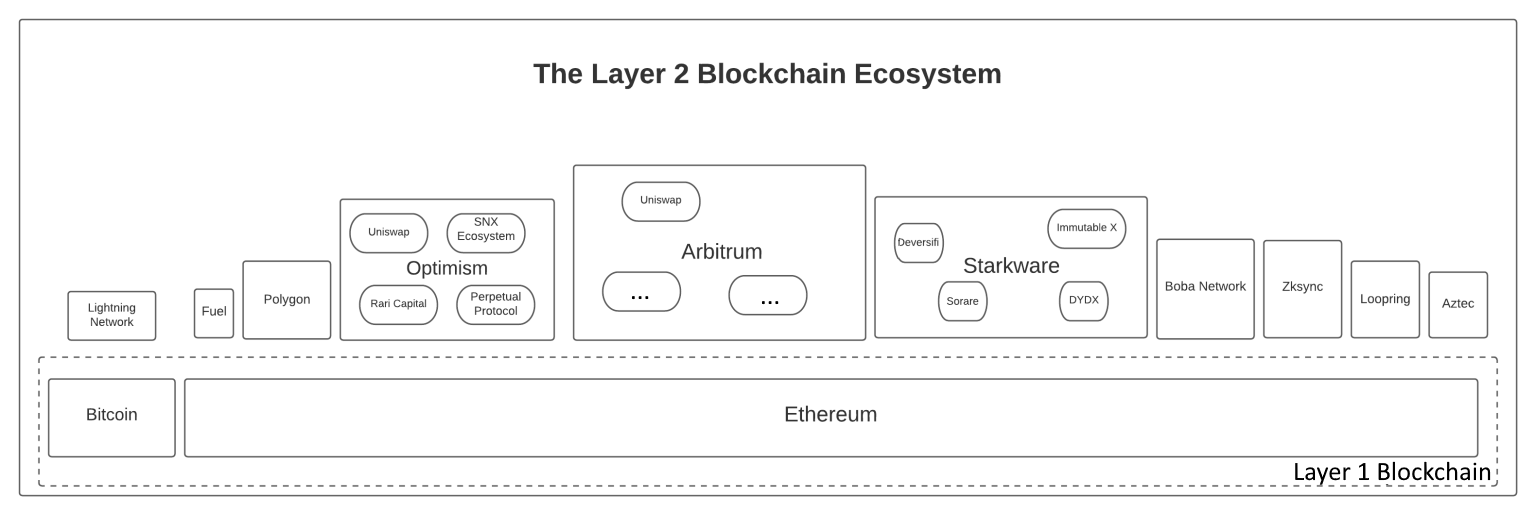
\includegraphics[scale=0.8]{./Pictures/Layer-2-Ecosystem-Map.png}
	\caption{Layer differentiation}
	\label{fig:Layer1_Layer2_comparison}
\end{figure}

\section{Optimistic Rollups}
We have already mentioned Arbitrum and how it is a possible Layer 2 solution to solve Ethereum's 
scaling and throughput problem, but we have yet to mention how it functions. 
Arbitrum uses a protocol that is based on optimistic rollups.
The name ``optimistic rollups'' is made up of two parts.

\subsection{Rollups}
The rollup half of optimistic rollups refers to the fact that only a rollup of the transaction data
gets posted on Layer 1. For example, if you create a smart contract on Arbitrum, you only have 
to post its hash, a hash of its state, and some other parameters on Layer 1. Doing so takes up 
much less space on the Ethereum blockchain, and having a 256-bit cryptographic hash of a smart
contract saved on the Ethereum blockchain ensures that the smart contract becomes immutable.
The illustration below in~\cref{fig:Optimistic_Rollups} shows a simplified version of how rollups 
work.

\subsection{Optimistic}
The optimistic half of optimistic rollups refers to how the rollups get posted on the Ethereum blockchain.
Any manager of a smart contract can assert that a state change has happened. Arbitrum is optimistic in
the sense that if nobody disputes this claim, the hash will be updated. However, if another user challenges
the claim within the given time frame of around a week, the protocol will go into the bisection protocol.
The bisection protocol takes a computation and splits it into two equal halves until a single false instruction 
is found. Once the single false instruction is found it can be sent to Layer 1 for evaluation to determine whether
the claim was valid or not.

This way in the optimistic scenario nothing ever has to be computed on chain and in the worst scenario only a single instruction
must be computed on chain.

\begin{figure}[h]
	\centering
	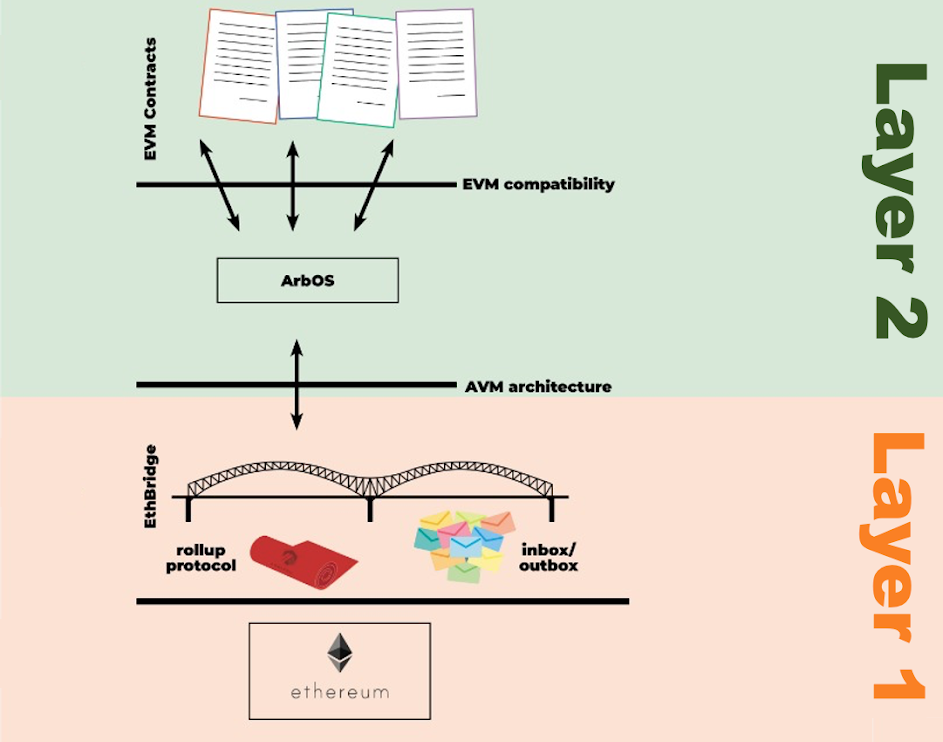
\includegraphics[scale=0.5]{./Pictures/Optimistic-Rollup.png}
	\caption{Optimistic Rollups}
	\label{fig:Optimistic_Rollups}
\end{figure}
  
\chapter{Background}

\section{Arbitrum White Paper}
The Arbitrum White Paper~\cite{ArbWP} was the first paper to propose optimistic rollups back in 2018. 
Over the following years, many of the details surrounding Arbitrum's implementation have changed and been refined. 
For example, in 2018 the main focus of Arbitrum was to increase privacy, scalability, and computational power of smart
contracts. Nowadays, the word ``privacy'' is nowhere to be found on Arbitrum's website or in its protocol description. 
Enhanced computational power still remains a priority, but the main focus has shifted to scalability and 
increasing throughput. The main idea of relying on optimistic rollups to achieve this goal, however
remains unchanged.

\section{Arbitrum Developers' Guide}
The Arbitrum developers' guide~\cite{ArbDevGuide} is the main source of information 
when it comes to Arbitrum today. It contains instructions on how to deploy smart 
contracts on Arbitrum. Information on how transaction fees are calculated. Descriptions 
of what smart contracts are running on Ethereum to make Arbitrum possible. 
Most, if not all, information related to Arbitrum today can be found there.

\section{Arbiscan}
Arbiscan is a website~\cite{Arbiscan} that allows its users to explore the Arbitrum 
blockchain without having to download the chain locally. This interface makes 
gathering data from the Arbitrum chain much easier and was the main tool we used 
when calculating the average transaction costs in Arbitrum.
The website is controlled by Arbitrum and was developed together with the help of 
the makers of Etherscan~\cite{ArbEthScan}.


\chapter{Analysing the cost differences}
In the following section we will be analysing the cost differences between Arbitrum and Ethereum
from both a theoretical and a practical point of view.

\section{Theoretical costs}
For finding out the theoretical cost differences between Arbitrum and Ethereum, 
our best reference was the Arbitrum developer guide~\cite{ArbDevGuide}. 
This contained detailed explanations of how Arbitrum calculates the cost of 
each transaction.

Similar to Ethereum, Arbitrum uses a measure called ArbGas. The idea behind ArbGas is 
identical to that of Ethereum. Since nodes have to verify a transaction, you pay them
in ArbGas. With the main difference being that ArbGas costs much less than Ethereum Gas 
and has a higher global limit. This way, you pay less for transactions and can perform larger
computations. However, Translating ArbGas into Ether is not as simple. 
Firstly, the Arbitrum network must calculate an estimate of the Ethereum gas fee.
We define this as
\[
	P := \text{Expected L1 Gas Price}.
\]
Afterwards, the transaction fee gets calculated via four different aspects:
\begin{itemize}
  \item L2 \textit{tx}: A base fee for each L2 transaction, to cover the cost of servicing a transaction
  \[
		\text{L2 } \textit{tx} = \frac{CP}{B}.
	\] 
	With $C$ being the L1 cost to submit a Batch to L1 and $B$ being the batch size.
	
  \item L1 \textit{calldata}: A fee per units of L1 calldata directly attributable to the transaction 
  (each non-zero byte of calldata is 16 units, and each zero byte of calldata is 4 units)
  \[
		\text{L1 } \textit{calldata} = P \cdot \text{calldata units}.
	\]
	
  \item \textit{computation}: A fee per unit of ArbGas used by the transaction.
  \[
		\textit{computation} = \text{ArbGas} \cdot \text{Base Price}
	\]
  With the base price being determined by the congestion of the Arbitrum network. 
  If the network is under heavy load, the base price gets multiplied by $9/8$. 
  If the network is under low load, the base price gets multiplied by $7/8$.
  Furthermore, the base price cannot go below $P/10'000$.
  
  \item \textit{storage}: A fee per location of EVM contract storage, based on the net increase in EVM storage due to the transaction.
  \[
		\textit{storage} = 2000 \cdot P \cdot \text{storage}
	\]
	You must pay 2'000 times the estimated L1 gas price per 256-Bit word of storage allocated. 
	Considering that in Ethereum you pay 20'000 gas per 256-bit word this implies that in Arbitrum
	you pay 10\% the expected Ethereum storage price.
\end{itemize}

If we add it all together we get
\[
	\text{Transaction Fee} = \text{L2 } \textit{tx} + \text{L1 } \textit{calldata} + \textit{computation} + \textit{storage}.
\]

Furthermore, if we assume that the base price is the minimum value of $P/10'000$ we get
\[
	\text{Transaction Fee} = P(\frac{C}{B} + \text{calldata units} + \frac{\text{Arb. Gas}}{10'000} + 2000 \cdot \text{storage}).
\]

\subsection{Example: Simple transaction}
	According to the Ethereum yellow paper~\cite{wood2014ethereum},
	for a simple transaction on Ethereum from one address to another you would have to pay 21'000 Gas.
	If we assume that the base fee was estimated correctly and no tip was given, we would get
	\[
		\text{Eth. cost} = 21,000 \cdot (\text{Base Fee} + \text{tip}) = 21'000 \cdot P.
	\]
	The same transaction on Arbitrum would cost us
	\[
		\text{Arb. cost} = P(\frac{C}{B} + 0 + \frac{21'000}{10'000} + 2000 \cdot 0) = \frac{CP}{B} + 2.1P.
	\]
	We can already see that the main cost comes from submitting the transaction to the L1 chain, while verifying the
	transaction would only cost us 2.1 Gas.
	If we take some reasonable values for $B$ and $C$ we would get $C = 1'200'000, B = 200$ 
	and then the cost becomes
	\[
		\text{Arb.cost} \approx 6'000 P + 2.1 P = 6002.1 P 
	\]
	In theory a basic Arbitrum transaction could cost around $6002.1/21'000 \approx 0.286$, 
	which is 28.6\% of the price of an Ethereum transaction. However, this value depends 
	heavily on $\frac{C}{B}$ and the percentage will only go down the more difficult 
	a transaction becomes. Consider the following
	\[
		\lim_{\text{Gas} \to \infty} \frac{P(6'000 + \text{Gas}/10'000)}{P \cdot \text{Gas}} = 
		\lim_{\text{Gas} \to \infty} \frac{6000 + \text{Gas}/10'000}{\text{Gas}} =
		\lim_{\text{Gas} \to \infty} \frac{6000}{\text{Gas}} + \frac{1}{10'000} =
		\frac{1}{10'000}
	\]
	This means that extremely computationally heavy transactions on Arbitrum could cost one 
	10'000th of the price they would on the Ethereum blockchain. In practice however, we can not
	let the ArbGas go to infinity since we would reach the ArbGas limit.
	
\section{Practical costs}
On august 31st, 2021, the Arbitrum Mainnet went online~\cite{ArbMainNet} 
and became accessible to the public. This development allowed us to not only theoretically 
analyse the cost differences but also analyse the practical cost differences between 
transactions happening on Arbitrum and transactions happening on Ethereum.

A motivation to do so was the fact that average transaction costs were readily available for 
Ethereum~\cite{EthTxCost}, while for Arbitrum there were no such services.
Furthermore, Arbiscan, the main blockchain explorer for Arbitrum, is made 
with the help of Etherscan~\cite{ArbEthScan} and both applications are close to identical in terms
of design and functionality. One of the key differences between the two sites is that Etherscan 
provides this information while Arbiscan does not. The exclusion of the average transaction costs
seems intentional from the side of Arbitrum.

\subsection{Data Gathering}
	Arbiscan provides an API for developers to gather and request data from the blockchain. 
	This was very helpful since it meant that we did not have to store the blockchain ourselves.
	Using the provided API seemed like the most logical way of gathering data until we realized
	that the provided calls were for very specific requests that involved exact account addresses 
	and not for the type of broad requests we needed to calculate average transaction costs.
	
	We instead opted to get the data ourselves from the Arbiscan website directly via html extraction.
	For this, we employed the use of urllib3~\cite{UrlLib3}, which would request and store the pages, and 
	BeautifulSoup~\cite{BS}, which was responsible for extracting the information.
	Arbiscan keeps track of the past 500'000 transactions with 50 transactions per page. 
	This amounts to around 2 weeks worth of transactions. 
	
	\subsection{Average calculation}
	The 500'000 entries were stored on a total of 10'000 pages. 
	Instead of processing all 10'000 pages and putting a large load on the Arbiscan servers 
	we opted to process a limited amount of pages chosen from the entire set.
	However, taking pages at random was also not an option. This would only 
	give us the average of 50 entries which would be prone to large variations. 
	We would instead create clusters of multiple pages and 	distribute theses clusters 
	evenly throughout the 10'000 pages.
	Using urllib we collected the data, parsed it, and then used the function 
	\textbf{numpy.mean(}costs\textbf{)} to get the average of each page and the average of
	each cluster. The function \textbf{numpy.meadian(}costs\textbf{)}, would be more robust
	to outliers but it would return the median value instead of an average value.
	\subsection{Plotting the data}
	Plotting the obtained average values in matplotlib gave us the average transaction fees over the course of the backlog.
	This can be seen below in~\cref{fig:Average_Arbitrum_Ether_Fees}
	
	\begin{figure}[h]
		\centering
		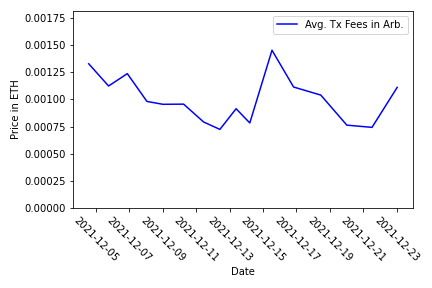
\includegraphics[scale=0.8]{./Pictures/arb_avg_eth1.png}
		\caption{Average Transaction Fees in Arbitrum in ETH}
		\label{fig:Average_Arbitrum_Ether_Fees}
	\end{figure}
	
	In~\cref{fig:Average_Arbitrum_Ether_Fees} you can see the price of an average transaction in the Arbitrum 
	network represented via the blue line. The y-axis shows us the average transaction costs in ETH and the x-axis
	shows us the respective dates on which these values were recorded. As we can see the backlog of 10'000 pages
	is enough to store 18 days worth of transactions. The average values of these transactions ranged from 
	0.0005 to 0.0015 ETH. We also see large variations between the data points. This could be due to the fact that the
	average is sensitive to outliers and we computed the average over 250 unfiltered entries.
	
	After obtaining the average transaction fees we needed to obtain historic Ethereum prices, as this would allow us 
	to plot the average transaction price in dollars. For this we used the python module cryptocompare. 
	Multiplying the costs with the Ether prices at the given dates gave us the graph 
	in~\cref{fig:Average_Arbitrum_USD_Fees}
	
	\begin{figure}[h]
		\centering
		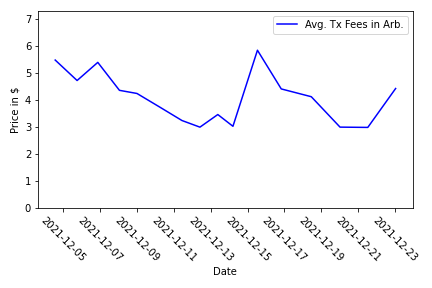
\includegraphics[scale=0.8]{./Pictures/arb_avg_usd1.png}
		\caption{Average Transaction Fees in Arbitrum in USD}
		\label{fig:Average_Arbitrum_USD_Fees}
	\end{figure}
	
	In~\cref{fig:Average_Arbitrum_USD_Fees} We see a graph which is practically identical to the graph
	in~\cref{fig:Average_Arbitrum_Ether_Fees}. The only difference being that the y-axis now represents the 
	average transaction costs in USD instead of ETH. The x-axis continues to show us
	us the respective dates on which these values were recorded. We see that an average
	Arbitrum transaction ranges from 3-6 USD. 
	We can also finally say that the expected transaction fee lies at around 4 USD.
	The strong variation in the graph remains even when multiplying the values 
	with historic Ethereum prices. This is mostly due to the Ethereum prices not 
	changing too drastically percentage-wise. 
	
	\clearpage
	\subsection{Comparison}
	To compare the average Arbitrum transaction fees with the average Ethereum transaction fees required us
	to first find a source of Ethereum transaction fees for given dates. For this we downloaded a csv file~\cite{ETHFees} 
	which only included Layer 1 transactions in the average calculation. Some sources started including Layer 2 transactions
	into the average calculations, but this would impact our comparison unfairly in favour of Ethereum. 
	Comparing the averages of the two gave us the following results seen in~\cref{fig:Arbitrum_Ethereum_Fees}.
	
	\begin{figure}[h]
		\centering
		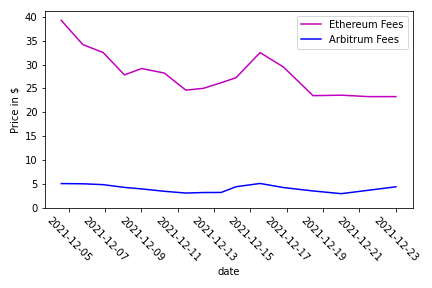
\includegraphics[scale=0.8]{./Pictures/arb_eth_fees1.png}
		\caption{Arbitrum Ethereum Comparison}
		\label{fig:Arbitrum_Ethereum_Fees}
	\end{figure}
	
	In~\cref{fig:Arbitrum_Ethereum_Fees} We see the results of our data gathering. The purple line
	represents the average Ethereum transaction costs, while the blue line represents the average
	Arbitrum transaction costs. Furthermore, the y-axis represents the given cost translated to USD,
	while the x-axis represents the dates on which these values were recorded.
	We can see that the average Arbitrum transaction lies at around 4-5 USD while the average
	Ethereum transaction averages at about 30 USD. This means that Arbitrum transactions cost
	around 85\% less compared to Ethereum transactions.
	
	we can also see that the Arbitrum network is not immune to fluctuations in the Ethereum network.
	On the 5th of December and on the 16th of December Ethereum had its highest transaction costs
	and so did Arbitrum.
	
	\clearpage
	Lastly, if we plot one minus the average Arbitrum costs divided by the average Ethereum costs we get 
	the following graph seen in~\cref{fig:Arbitrum_Ethereum_Save}
	
	\begin{figure}[h]
		\centering
		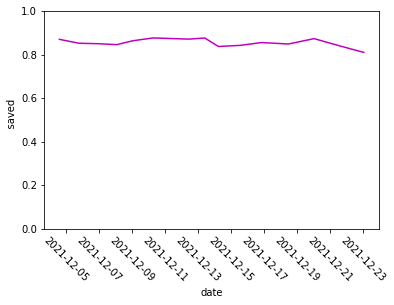
\includegraphics[scale=0.8]{./Pictures/arb_eth_save1.png}
		\caption{Arbitrum Cost Saved}
		\label{fig:Arbitrum_Ethereum_Save}
	\end{figure}
	
	The purple line represents the calculated ratio between Arbitrum and Ethereum transactions. The y-axis contains
	values between 0 and 1. The x-axis continues to represent the dates on which these values were recorded.
	We can see that executing a transaction on the Arbitrum network would save us on average more than 80\% of 
	the transaction costs.

\chapter{Conclusion}
\label{ch:conclusion}

This report set out to give a clear comparison and provide concrete numbers 
between transactions on Layer 1, which happen on the
Ethereum blockchain, and transactions on Layer 2, which happen on Arbitrum.
For this, we first had to extract data from the Arbitrum blockchain and calculate the 
average transaction fees ourselves, since the Arbitrum blockchain explorer refused to provide this data. 

When comparing both averages directly with each other, we can see that the average cost 
per transaction on the Arbitrum network is much lower than that of an average transaction on the
Ethereum network. These results fit rather well with our theoretical estimate. There, we calculated that
an Arbitrum transaction would cost less than 70\% the amount that an equivalent Ethereum transaction 
would. Our results say that Arbitrum transactions cost 80\% less. Overall the Practical implementation
of Arbitrum coincides with the Theoretical implementation in terms of transaction fees.

The only questionable thing remains that Arbiscan does not display the average transaction fees,
although this data is readily available to them. It highlights the strong centralization of Arbitrum 
and the power they hold over the network. Restricting the flow of information and instead only
showing extremely favourable information is not in the spirit of decentralized networks.

% The bibliography appears after any appendix.

% using BiBTeX is required
\bibliography{Report}

% any bibstyle is fine, this one give particularly compact output 
\bibliographystyle{ieeetran}
\end{document}
